\section{Background and Literature Review}
\label{sec:background-literature-review}

The literature background is used here to narrow the modelling problem, not to
catalog every hemodynamic model class. Stenotic flow creates localized geometry,
velocity, pressure, and wall-interaction effects. Three-dimensional CFD and FSI
resolve those effects most directly, but require detailed geometry, material
data, boundary histories, and substantially higher computational cost. Reduced
models are therefore useful when the research question concerns distributed
pressure--flow behavior, repeatable numerical studies, or parameter scans, but
their predictions depend on declared averaging, closure, wall, geometry, and
boundary assumptions.

\subsection{Continuum and Constitutive Assumptions}
\label{subsec:continuum-constitutive-assumptions}

This section moves from the macroscopic scale assumption, 
to continuum field variables, to balance-law vocabulary,
and finally to Newtonian versus generalized-Newtonian stress closures.

\subsubsection{Physiological Scale Boundary}
\label{subsubsec:physiological-scale-boundary}

The present work is posed at the macrocirculatory arterial scale. 
At this scale, blood is commonly modeled as a viscous fluid whose bulk behavior
can be described by continuum mechanics. The goal is not to resolve the effects of individual
blood cells, platelets, or plasma constituents but rather to predict
macroscopic observables such as pressure, flow rate, pressure drop, and
pressure ratio.
\cite[Sec.~1.1.2, pp.~9–10]{KopplHelmig2023DimensionReducedModeling}
\cite[Sec.~1.1.3, pp.~12–14]{KopplHelmig2023DimensionReducedModeling}.

\subsubsection{Blood as a Continuum}
\label{subsubsec:blood-as-a-continuum}

Consider a time-dependent family of spatial fluid domains. For a final time
$T_{\mathrm{final}}>0$, use
$I_T\defined(0,T_{\mathrm{final}})$ for interior-time PDE statements and
$\overline{I}_T\defined[0,T_{\mathrm{final}}]$ for initial data and flow maps.
Define
\begin{flalign*}
    \quad \begin{cases}
     \OmgBt \defined \{\vx \in \R^3 : \vx \text{ lies inside the vessel at time } t\} \\
     \mathcal{Q}_T \defined \{(t,\vx):t\in I_T,\ \vx\in\OmgBt\},
    \end{cases}&&
\end{flalign*}
where the reference configuration is denoted $\OmgB(0)$, the current
configuration is $\OmgBt$, and the space-time fluid domain is $\mathcal{Q}_T$.
This domain notation is the one collected in
Appendix~\ref{app:mathematical-notation}; boundary and function-space
conventions are summarized in Appendix~\ref{app:mathematical-foundations}. In
this report, the continuum assumption is a large-vessel idealization: individual
blood cells, platelets, and plasma constituents are not resolved, and blood
velocity, pressure, density, and Cauchy stress are represented by sufficiently
regular fields on $\mathcal{Q}_T$. Cellular-scale effects may enter only
through later constitutive choices
\cite[Part~I, Ch.~1, Secs.~1.1--1.2, pp.~4--5]{hemodynamics}
\cite[Secs.~1.1.3 and~3.2, pp.~12--14 and~46--47]{KopplHelmig2023DimensionReducedModeling}.
The continuum setup is as follows: Remark~\ref{rmk:eulerian-lagrangian},
Definition~\ref{def:material-derivative},
Definitions~\ref{def:material-density-preservation}--\ref{def:incompressible-flow},
Definitions~\ref{def:linear-momentum-balance}--\ref{def:linear-momentum-balance-strong},
and Definitions~\ref{def:fluidsmodel}--\ref{def:incompressible-stress-tensor}
fix the assumptions used in the model hierarchy.


\subsubsection{Blood Dynamics}
\label{subsubsec:blood-dynamics}

This subsection fixes the kinematic vocabulary used by the later continuum and
reduced-order models.
For $t\in\overline{I}_T$, let
$\La_t:\OmgB(0)\to\OmgB(t)$ be an orientation-preserving
diffeomorphism with $\det\nabla_{\vxi}\La_t>0$.
As a standing assumption, the family $\La_t$ has the time and space regularity
needed to differentiate $\nabla_{\vxi}\La_t$ and
$\det\nabla_{\vxi}\La_t$ in the classical identities below and in
Appendix~\ref{app:continuum-derivation-details}.
It carries each material label $\vxi$ to its current location
$\vx(t,\vxi)=\La_t(\vxi)$.
The Eulerian velocity field $\vu:\mathcal{Q}_T\to\R^3$ satisfies
\begin{flalign*}
    \quad \partial_t\La_t(\vxi)=\vu(t,\La_t(\vxi)). &&
\end{flalign*}
Figure~\ref{fig:lagrangian-eulerian-map} illustrates this Lagrangian--Eulerian
notation.

\begin{figure}[!htb]
    \centering
    \captionsetup{aboveskip=2pt,belowskip=2pt}
    \figtikz{lagrangian-eulerian-map}
    \caption{%
        Lagrangian and Eulerian descriptions. The flow map
        $\La_t:\OmgB(0)\to\OmgBt$ carries the material label
        $\vxi\in\OmgB(0)$ to its current position
        $\vx(t,\vxi)\in\OmgBt$. The Eulerian velocity $\vu(t,\vx)$
        is the velocity of whichever particle currently sits at
        $(t,\vx)$; the Lagrangian velocity is
        $\vuhat(t,\vxi)=\partial_t\vx(t,\vxi)=\vu(t,\La_t(\vxi))$,
        and trajectories $T_{\vxi}$ are generated by the velocity field $\vu$.}
    \label{fig:lagrangian-eulerian-map}
\end{figure}

\begin{remark}[Eulerian vs. Lagrangian]
    \label{rmk:eulerian-lagrangian}
    The Eulerian description views fields such as $\phi(t,\vx)$ or
    $\vu(t,\vx)$ at fixed spatial locations. The Lagrangian description follows
    material particles $\vxi$ along trajectories generated by the velocity field and views fields as functions of the
    material label $\vxi$ and time $t$, such as $\widehat{\phi}(t,\vxi)=\phi(t,\La_t(\vxi))$ or
    $\vuhat(t,\vxi)=\vu(t,\La_t(\vxi))$. The flow map $\La_t$ is the change of
    variables between these descriptions, and the trajectory of a particle with
    label $\vxi$ is the characteristic curve
    $t\mapsto \vx(t;\vxi)=\La_t(\vxi)$. Where defined, the inverse
    $\La_t^{-1}$ maps an Eulerian location back to its material label.
\end{remark}

Under the standard assumption that the prescribed velocity field is continuous in time and uniformly Lipschitz in space, particle trajectories exist uniquely and depend continuously on their initial labels; see \cite[Ch.~2]{Teschl2012OrdinaryDifferentialEquations}. This is a trajectory-level ODE result and should not be confused with Navier--Stokes well-posedness.

\begin{definition}[Material derivative]
    \label{def:material-derivative}
    For $\phi\in C^1(\mathcal{Q}_T)$, the material derivative is the derivative
    of $\phi$ along a particle trajectory:
    \begin{flalign*}
        \quad D_t\phi(t,\vx)
        \defined
        \frac{d}{dt}\phi(t,\La_t(\vxi))
        =
        \partial_t\phi(t,\vx)+\vu(t,\vx)\cdot\nabla\phi(t,\vx),
        \qquad \vxi=\La_t^{-1}(\vx). &&
    \end{flalign*}
    For vector fields, $D_t$ is applied componentwise.
\end{definition}

Let $\vFhat_t=\nabla_{\vxi}\La_t$ be the deformation gradient and
$\Jhatdet_t=\det\vFhat_t$ the Jacobian determinant. In Eulerian notation this
is written $\Jdet_t(\vx)=\det\vFhat_t(\La_t^{-1}(\vx))$. The standard Jacobian evolution law $D_t\Jdet_t=\Jdet_t\,\Div\vu$ is used implicitly below; derivation details are deferred to Appendix~\ref{app:continuum-derivation-details}.

\begin{theorem}[Reynolds Transport Theorem]
    \label{thm:reynolds-transport}
    Let $V(t)=\La_t(V(0))$ be a bounded material volume with Lipschitz boundary.
    If $\phi\in C^1(\mathcal{Q}_T)$, then
    \begin{flalign*}
        \quad \frac{d}{dt}\int_{V(t)}\phi\,\dx
        &=
        \int_{V(t)}\left(D_t\phi+\phi\,\Div\vu\right)\dx \\
        &=
        \int_{V(t)}\left(\partial_t\phi+\Div(\phi\vu)\right)\dx. &&
    \end{flalign*}
\end{theorem}

Proof-level details for Theorem~\ref{thm:reynolds-transport} and the momentum balance below are found
in Appendix~\ref{app:continuum-derivation-details}.

\subsubsection*{Continuum assumptions retained in the main model}

Let the 3D velocity, pressure, and density fields be
\begin{flalign*}
    \quad \vu:\mathcal{Q}_T\to\R^3,\qquad
    p:\mathcal{Q}_T\to\R,\qquad
    \rho:\mathcal{Q}_T\to\R^+. &&
\end{flalign*}
The balance-law vocabulary developed below permits variable density. The reduced arterial models considered later adopt the constant-density specialization $\rho\equiv\rho_0>0$, which is standard for large-vessel incompressible blood-flow models.

The domains and material control volumes are assumed regular enough for traces,
outward unit normals, and the divergence theorem; Lipschitz boundaries are
sufficient for the integral manipulations used here; see
Convention~\ref{conv:foundation-standing-regularity} in
Appendix~\ref{app:mathematical-foundations}.

\begin{definition}[Material density preservation]
    \label{def:material-density-preservation}
    A flow has material density preservation if density is preserved along
    particle trajectories:
    \begin{flalign*}
        \quad D_t\rho=0. &&
    \end{flalign*}
\end{definition}

\begin{definition}[Incompressible flow]
    \label{def:incompressible-flow}
    A flow is incompressible, or volume preserving, if material volumes are
    preserved. With $\La_0=\mathrm{Id}$ this is equivalent to
    \begin{flalign*}
        \quad \Jdet_t\equiv 1
        \quad \Longleftrightarrow \quad
        \Div\vu=0. &&
    \end{flalign*}
\end{definition}

\begin{remark}[Divergence-free condition]
    \label{rmk:incompressibility-divergence-free}
    Mass conservation gives
    \begin{flalign*}
        \quad \partial_t\rho+\Div(\rho\vu)=0
        \quad \Longleftrightarrow \quad
        D_t\rho+\rho\Div\vu=0. &&
    \end{flalign*}
    In the constant-density model used for incompressible Navier--Stokes,
    $\rho\equiv\rho_0>0$, so mass conservation reduces to
    $\Div\vu=0$ in $\mathcal{Q}_T$.
\end{remark}

\begin{definition}[Linear momentum balance]
    \label{def:linear-momentum-balance}
    For a material fluid element $V(t)\subset\OmgBt$, the linear momentum balance is
    \begin{flalign*}
        \quad
        \frac{d}{dt}\int_{V(t)}\rho\vu\,dV
        =
        \int_{\partial V(t)}\vT\nhat\,dS
        +
        \int_{V(t)}\rho\vfb\,dV, &&
    \end{flalign*}
    where $\vT$ is the Cauchy stress tensor and $\vfb$ is body force per unit mass.
\end{definition}

\begin{definition}[Strong momentum balance]
    \label{def:linear-momentum-balance-strong}
    Under the regularity and mass-balance assumptions above, the local momentum
    balance is
    \begin{flalign*}
        \quad
        \rho\left(\partial_t\vu+(\vu\cdot\nabla)\vu\right)
        =
        \Divbf(\vT)+\rho\vfb,
        \qquad \text{in } \OmgBt. &&
    \end{flalign*}
\end{definition}

The stress law closes the momentum equation. Let the rate-of-deformation tensor be
\begin{flalign*}
    \quad \vct{D}(\vu)\defined
    \frac{1}{2}\left(\nabla\vu+\nabla\vu^\top\right). &&
\end{flalign*}

\begin{definition}
    \label{def:newtonian-fluid}
    A fluid is Newtonian if, after separating the pressure contribution, its
    viscous stress depends linearly on the rate-of-deformation tensor
    $\vct{D}(\vu)$.
\end{definition}

\begin{remark}[Blood isotropy justification]
    \label{rmk:blood-isotropy-justification}
    Blood is often modeled as an isotropic continuum fluid at large-vessel
    scales. This is a closure assumption for averaged behavior, not a microscopic
    statement about cells suspended in plasma. The cited sources support the
    scale and rheology caveat--nearly constant large-vessel relative viscosity
    versus diameter- and hematocrit-dependent apparent viscosity in small tubes--not
    a direct cellular-level isotropy claim
    \cite[Sec.~1.1.3, Fig.~1.14, pp.~12--14; Sec.~3.2, pp.~46--47]{KopplHelmig2023DimensionReducedModeling}
    \cite[Abstract; pp.~H1770--H1772]{bviscosity}.
\end{remark}

\begin{remark}[Isotropic constitutive response]
    \label{rmk:isotropy-implication}
    An isotropic fluid has a constitutive response that is independent of the chosen coordinate system. Consequently, the Cauchy stress depends on coordinate-free invariants of $\vct{D}(\vu)$ rather than on a particular basis.
\end{remark}

\begin{definition}[Newtonian, isotropic constitutive law]
    \label{def:fluidsmodel}
    For a Newtonian, isotropic fluid,
    \begin{flalign*}
        \quad \vT=-p\,\ident+2\eta\,\vct{D}(\vu)
        +\lambda\,\Div(\vu)\,\ident, &&
    \end{flalign*}
    where $\eta$ is the dynamic viscosity and $\lambda$ is the coefficient of the
    volumetric-viscous term.
\end{definition}

\begin{definition}[Incompressible stress tensor]
    \label{def:incompressible-stress-tensor}
    When $\Div\vu=0$, the Newtonian incompressible Cauchy stress is
    \begin{flalign*}
        \quad \vT=-p\,\ident+2\eta\,\vct{D}(\vu). &&
    \end{flalign*}
\end{definition}

More general models allow viscosity to vary with shear rate. For generalized Newtonian blood models, the dynamic viscosity is allowed to depend on the local deformation-rate magnitude
\cite[Part~I, Ch.~1, Secs.~2.7--3.1, pp.~16--19]{hemodynamics}.
A standard constitutive form is
\begin{flalign*}
    \quad \dot{\gamma}\defined\sqrt{2\vct{D}(\vu):\vct{D}(\vu)}, &&
\end{flalign*}
\begin{flalign*}
    \quad \vT=-p\,\ident
    +2\eta_{\mathrm{eff}}(\dot{\gamma})\vct{D}(\vu). &&
\end{flalign*}
Here
\begin{flalign*}
    \quad \norm{\vct{D}(\vu)}^2 \defined \vct{D}(\vu):\vct{D}(\vu)
    =\sum_{i,j}D_{ij}(\vu)^2 &&
\end{flalign*}
is the pointwise Frobenius norm squared. When a source writes the viscosity as a
function of \(D:D\) or \(|D|_{\mathrm F}^2\), this report translates it
through the scalar shear-rate convention above.
Here $\eta_{\mathrm{eff}}$ is an effective dynamic viscosity. Kinematic
viscosity is $\nu=\eta/\rho$ after division by density.
The Newtonian incompressible model is recovered from this generalized
Newtonian form when $\eta_{\mathrm{eff}}$ is constant.

\begin{remark}[Newtonian Blood Justification]
    \label{rmk:newtonian-justification}
    For large arteries, empirical studies suggest that apparent viscosity is often
    approximately constant across the relevant operating range, motivating the
    Newtonian approximation in many reduced-order hemodynamic models. However,
    diameter-dependent, hematocrit-dependent, and shear-dependent effects become
    increasingly important in smaller vessels and low-shear regions
    \cite[Sec.~1.1.3, pp.~12–14]{KopplHelmig2023DimensionReducedModeling}
    \cite{bviscosity}.
\end{remark}

\subsection{Governing Equations and Model Hierarchy}
\label{subsec:governing-equations-model-hierarchy}

The continuum assumptions of
Section~\ref{subsec:continuum-constitutive-assumptions} lead to a layered
modeling hierarchy. In particular,
Assumption~\ref{ass:blood-dynamics-kinematic-setting} supplies the flow map,
material volumes, and continuum fields on which the conservation laws act. The
high-fidelity starting point is the incompressible Navier--Stokes or
generalized-Newtonian system on a three-dimensional lumen. The report then uses
cross-sectional reduction to identify the selected 1D area-flow variables and
to state the closure assumptions that must be fixed before any reduced
numerical study is interpreted.

\subsubsection{Conservation Laws and Navier--Stokes Specialization}
\label{subsubsec:conservation-laws}

The governing equations originate from conservation of mass and linear momentum
applied to material volumes under
Assumption~\ref{ass:blood-dynamics-kinematic-setting}, followed by the
constant-density incompressible specialization. The derivation details and
row-divergence convention are recorded in
Appendix~\ref{app:continuum-derivation-details} and
Definition~\ref{def:foundation-differential-operator-conventions}.
Figure~\ref{fig:ns-derivation-map} summarizes the route from these balance laws
to the forms used in the report
\cite[Part~I, Ch.~1, Secs.~2.2--3.1, pp.~11--19; Part~IV, Ch.~1,
Sec.~1.1, pp.~380--383]{GaldiEtAl2008HemodynamicalFlows}
\cite[Sec.~6]{QuarteroniFormaggia2004CardiovascularModeling}.

\begin{figure}[!htb]
    \centering
    \captionsetup{aboveskip=2pt,belowskip=2pt}
    \figtikz{ns-derivation-map}
    \caption{From the blood-dynamics setting to incompressible
    Navier--Stokes. The flow map and material-volume assumptions support the
    conservation statements. Mass conservation reduces to $\Div\vu=0$ under
    constant density. Momentum balance closes through the Cauchy stress law;
    the Newtonian limit uses constant dynamic viscosity, while the
    generalized-Newtonian form keeps $\eta_{\mathrm{eff}}(\dot\gamma)$
    explicit.}
    \label{fig:ns-derivation-map}
\end{figure}

With this kinematic setting fixed, mass conservation for the constant-density
incompressible model gives
\begin{flalign*}
    \quad \Div\vu = 0 \qquad \text{in } \OmgBt. &&
\end{flalign*}
Linear momentum conservation balances inertia, pressure, viscous stress, and
body forces:
\begin{flalign*}
    \quad
    \rho \left(\pd_t \vu+(\vu\cdot\nabla)\vu\right)
    \equals \Divbf(\vT)+\rho\vfb. &&
\end{flalign*}
Throughout the Navier--Stokes statements below, \(\vfb\) denotes body force per
unit mass, so \(\rho\vfb\) is the corresponding body force per unit volume.

\begin{definition}[Conservative incompressible Navier--Stokes]
    \label{def:nsconservative}
    On \(\OmgBt\), the constant-density Newtonian system may be written in
    conservative tensor-divergence form as
    \begin{flalign*}
        \quad & \begin{cases*}
            \pd_t (\rho \vu)
            + \Divbf(\rho \vu\otimes\vu)
            =
            -\nabla p+\Divbf(2\eta\vct{D}(\vu))+\rho\vfb, \\
            \Div\vu=0,\qquad \rho\equiv\rho_0>0.
        \end{cases*} &&
    \end{flalign*}
\end{definition}

For constant density and divergence-free velocity,
\(\Divbf(\rho\vu\otimes\vu)=\rho(\vu\cdot\nabla)\vu\). Thus the same Newtonian
momentum equation can be read in advective form.

\begin{definition}[Generalized-Newtonian incompressible Navier--Stokes]
    \label{def:NSEquations}
    For an incompressible generalized-Newtonian fluid, use the shear-rate
    convention
    \begin{flalign*}
        \quad
        \dot{\gamma}\defined\sqrt{2\vct{D}(\vu):\vct{D}(\vu)}. &&
    \end{flalign*}
    The velocity \(\vu\), pressure \(p\), body force per unit mass \(\vfb\), and constant
    density \(\rho\equiv\rho_0>0\) satisfy
    \begin{flalign*}
        \quad & \begin{cases*}
            \rho\big(\pd_t \vu+(\vu\cdot\nabla)\vu\big)
            =
            -\nabla p
            +\Divbf\!\Big(
                2\eta_{\mathrm{eff}}(\dot\gamma)\vct{D}(\vu)
            \Big)
            +\rho\vfb, \\
            \Div\vu=0.
        \end{cases*} &&
    \end{flalign*}
\end{definition}

\begin{definition}[Density-scaled generalized Navier--Stokes]
    \label{def:density-scaled-generalized-ns}
    With
    \(\nu_{\mathrm{eff}}(\dot\gamma)
    \defined\eta_{\mathrm{eff}}(\dot\gamma)/\rho\), the divided-by-density form
    is
    \begin{flalign*}
        \quad & \begin{cases*}
            \pd_t \vu+(\vu\cdot\nabla)\vu
            =
            -\rho^{-1}\nabla p
            +\Divbf\!\Big(
                2\nu_{\mathrm{eff}}(\dot\gamma)\vct{D}(\vu)
            \Big)
            +\vfb, \\
            \Div\vu=0.
        \end{cases*} &&
    \end{flalign*}
\end{definition}
The density-scaled form is particularly useful for numerical simulations,
because it separates the convective ($(\vu\cdot\nabla)\vu$) and diffusive /
viscous-stress
($\Divbf(2\nu_{\mathrm{eff}}(\dot\gamma)\vct{D}(\vu))$) contributions in the
momentum equation, allowing for more straightforward numerical treatment of
each term independently.
\begin{definition}[Newtonian incompressible Navier--Stokes]
    \label{def:newtonian-incompressible-ns}
    If \(\eta_{\mathrm{eff}}\equiv\eta\) is constant, then sufficiently smooth
    divergence-free velocity fields satisfy
    \(\Divbf(2\eta\vct{D}(\vu))=\eta\del\vu\). The Newtonian equations are
    \begin{flalign*}
        \quad & \begin{cases*}
            \rho\big(\pd_t \vu+(\vu\cdot\nabla)\vu\big)
            =
            -\nabla p+\eta\del\vu+\rho\vfb, \\
            \Div\vu=0,
        \end{cases*}
        \qquad
        \begin{cases*}
            \pd_t \vu+(\vu\cdot\nabla)\vu
            =
            -\rho^{-1}\nabla p+\nu\del\vu+\vfb, \\
            \Div\vu=0,
        \end{cases*}
        &&
    \end{flalign*}
    where \(\nu\defined\eta/\rho\).
\end{definition}

Thus the 3D PDE tier is not introduced independently: flow maps and material
volumes support Reynolds transport, Reynolds transport gives mass and momentum
balance, the Cauchy stress law closes momentum, and incompressibility selects
the Navier--Stokes systems above.

\begin{definition}[Navier--Stokes residual notation]
    \label{def:standard-form-ns}
    The density-scaled generalized system can be summarized by a momentum
    residual operator:
    \begin{flalign*}
        \quad & \begin{cases*}
            \mathcal{R}_{\mathrm{NS}}
            (\pd_t \vu,\nabla\vu,\nabla p,\vu,p;\rho,\nu_{\mathrm{eff}})
            =\vfb, \\
            \Div\vu=0.
        \end{cases*} &&
    \end{flalign*}
\end{definition}

\begin{remark}[Navier--Stokes system classification]
    \label{rmk:ns-system-classification}
    Navier--Stokes is a nonlinear coupled PDE system. The unknowns are the
    three velocity components and pressure. The convective term transports
    momentum, the pressure gradient enforces incompressibility, and the viscous
    term diffuses momentum through the stress tensor.
\end{remark}

\subsubsection{Boundary Data and Well-Posedness Context}
\label{subsubsec:boundary-initial-data-vocabulary}

For a single-vessel three-dimensional domain, write the boundary decomposition
\begin{flalign*}
    \quad
    \partial\OmgBt
    =
    \Gamma_{\mathrm{in}}(t)\cup
    \Gamma_{\mathrm{out}}(t)\cup
    \Gamma_w(t). &&
\end{flalign*}
Here \(\Gamma_{\mathrm{in}}(t)\) denotes an inlet portion where a velocity,
flow-rate, or profile condition may be prescribed. The outlet portion
\(\Gamma_{\mathrm{out}}(t)\) carries pressure, traction, or reduced downstream
network data. The wall portion \(\Gamma_w(t)\) carries either a no-slip or
no-penetration condition for a fixed-wall continuum model, or a wall-law or
structure closure when wall motion is retained. A complete initial-boundary
value problem also states \(\vu(0,\cdot)=\vu_0\), the domain, forcing,
compatibility assumptions, and the solution class.

\begin{remark}[Global regularity context]
    \label{rmk:global-regularity}
    For smooth, spatially localized initial data in three dimensions, global
    existence and smoothness for Navier--Stokes remains an open Clay Millennium
    Prize problem \cite[Problem statement]{ClayMathematicsInstitute2022NavierStokesEquation}. This is
    mathematical context for the 3D continuum model, not a direct limitation of
    the controlled reduced 1D solver introduced below.
\end{remark}

Well-posedness results for a three-dimensional Navier--Stokes
initial-boundary value problem are problem-specific: the statement must fix the
domain class, boundary conditions, forcing, compatibility assumptions,
initial-data space, solution class, and time horizon. The present report uses
that vocabulary only as PDE background for the model hierarchy. It does not use
the Clay global-regularity problem as support for a local theorem, and it does
not prove a well-posedness result for the moving arterial domain or for the
reduced numerical solver. The domain and function-space notation relevant to
such statements is summarized in Appendix~\ref{app:mathematical-foundations};
coordinate and energy background is collected in
Appendix~\ref{app:ns-coordinate-details}.

\subsubsection{Cross-Sectional Reduction and Selected 1D Model}
\label{subsubsec:cross-sectional-reduction-selected-1d-model}

The 1D model reduces the spatial dimension by assuming that the vessel has a
distinguished axial direction and that pressure and velocity can be averaged
over cross-sections. This keeps pulse-wave and pressure-drop structure while
discarding secondary flow, separation, recirculation, and resolved wall
traction. The reduction follows standard compliant-artery and
dimension-reduced modeling arguments
\cite[Sec.~2, pp.~253--257]{FormaggiaEtAl2003OneDimensionalBloodFlow}
\cite[Ch.~3, Secs.~3.2 and~3.6]{KopplHelmig2023DimensionReducedModeling}
\cite[Sec.~3, pp.~24--26]{ShiEtAl2011BloodFlowModelReview}.
The reduced variables \(A\), \(Q\), \(\bar u\), and \(p_{\mathrm g}\) should
therefore be read as cross-sectional outputs of the continuum fields under
additional averaging, geometry, wall-law, and profile assumptions, not as
independent replacements for the blood-dynamics setting above.

\begin{figure}[!htb]
    \centering
    \captionsetup{aboveskip=2pt,belowskip=2pt}
    \figtikz{compliant-vessel}
    \caption{Compliant-vessel notation for the 1D reduction. The physical
    lumen \(\OmgBt\) is represented by a straightened averaging domain with
    cross-section \(S(z,t)\), area \(A(z,t)\), flow \(Q(z,t)\), radius
    \(R(z,t)\), and mean gauge pressure \(p_{\mathrm g}(z,t)\).}
    \label{fig:compliant-vessel-reduction}
\end{figure}

\begin{assumption}[Straight single-vessel geometry]
    \label{ass:1d-straight-vessel-geometry}
    The selected 1D lane assumes a vessel of length \(L\) aligned with the
    \(z\)-axis and a circular cross-section with radius \(R(z,t)\). For
    \(0<z<L\), \(S(z,t)\) is the interior cross-section used for averaging, not
    a boundary component of the open lumen.
\end{assumption}

\begin{definition}[Section-averaged 1D fields]
    \label{def:section-averaged-1d-fields}
    The retained reduced variables are
    \begin{flalign*}
        \quad A(z,t) &\defined \int_{S(z,t)} 1 \, dS, &&
            \text{cross-sectional area}, \\
        \quad Q(z,t) &\defined \int_{S(z,t)} u_z \, dS, &&
            \text{volumetric flow rate}, \\
        \quad \bar u(z,t) &\defined \frac{Q(z,t)}{A(z,t)}, &&
            \text{mean axial velocity}, \\
        \quad p_{\mathrm g}(z,t) &\defined \frac{1}{A(z,t)}
            \int_{S(z,t)} p_{3D,\mathrm g} \, dS, &&
            \text{mean gauge pressure}.
    \end{flalign*}
    Here \(p_{3D,\mathrm g}\) is continuum pressure in the wall-law gauge
    frame. The pressure-reference convention for reduced ratios is fixed
    separately in Convention~\ref{conv:appendix-pressure-reference-ratio}.
\end{definition}

\begin{definition}[Wall and FSI closure catalog]
    \label{def:wall-fsi-closure-catalog}
    The descriptor \(\mathcal W\) records how the wall or wall-reduced
    mechanics are closed. It is independent of the rheology descriptor
    \(\mathcal R\): \(\mathcal R\) changes the stress or effective-viscosity
    law, while \(\mathcal W\) changes whether the vessel wall is fixed,
    algebraically reduced, coupled to another model tier, or resolved as a
    structure.
    \begin{center}
    \footnotesize
    \begin{tabularx}{\textwidth}{@{}
        >{\raggedright\arraybackslash}p{0.21\textwidth}
        >{\raggedright\arraybackslash}X
        >{\raggedright\arraybackslash}X
        @{}}
        \toprule
        \textbf{Closure descriptor}
            & \textbf{Wall information retained}
            & \textbf{Reading in this report} \\
        \midrule
        \(\mathcal W_{\mathrm{rigid}}\)
            & Fixed or prescribed wall geometry; no structural state is solved
            & A fixed-wall continuum or rigid-tube reduced baseline. This is not
            an FSI model, even when no-slip or no-penetration wall data are
            imposed. \\
        \(\mathcal W_{\mathrm{elastic1D}}\)
            & Dynamic area \(A(z,t)\), gauge pressure \(p_{\mathrm g}(A,z,t)\),
            reference area \(A_0(z)\), wall stiffness \(\beta(z)\), and
            external pressure
            & The selected single-vessel model. Wall mechanics are reduced to a
            pressure--area law, wave speed, elastic potential, and geometry
            source; no separate structural PDE is solved. \\
        \(\mathcal W_{\mathrm{multiscale}}\)
            & Interface pressure, flow, traction, or characteristic data coupling
            0D, 1D, and 3D model tiers
            & A boundary or coupling model requiring a separate interface and
            stability contract; it is not implied by the single-vessel
            flux/source notation. \\
        \(\mathcal W_{\mathrm{resolvedFSI}}\)
            & Fluid velocity and pressure plus wall displacement, wall velocity,
            structural stress, and interface conditions
            & A full moving-wall FSI PDE system. It is a comparison tier for this
            report, not the active model in the first \(T=1\) study. \\
        \bottomrule
    \end{tabularx}
    \end{center}
    This separation follows the standard distinction between reduced compliant
    vessel models, geometrical multiscale coupling, and resolved FSI models
    \cite[Sec.~2, pp.~253--257]{FormaggiaEtAl2003OneDimensionalBloodFlow}
    \cite{QuarteroniVeneziani2003GeometricalMultiscale}
    \cite{FormaggiaEtAl2007FSICoupling}.
\end{definition}

\begin{definition}[Closed 1D area-flow model]
    \label{def:closed-1d-area-flow-model}
    For \(\mathcal W=\mathcal W_{\mathrm{elastic1D}}\) and an incompressible
    fluid with density \(\rho\), the working compliant single-vessel model is
    written with the composite axial pressure derivative
    \begin{flalign*}
        \quad
        \frac{d}{dz}p_{\mathrm g}(A(z,t),z,t)
        =
        \pd_A p_{\mathrm g}(A,z,t) \pd_z A
        +
        \left.\pd_z p_{\mathrm g}(A,z,t)\right|_A . &&
    \end{flalign*}
    The reduced balance law is
    \begin{flalign*}
        \quad \pd_t A
        + \pd_z Q
        &= 0, \numberthis\label{eq:1d-mass-aq} && \\
        \quad \pd_t Q
        + \pd_z
            \left(\alpha \frac{Q^2}{A}\right)
        + \frac{A}{\rho}\frac{d}{dz}p_{\mathrm g}(A(z,t),z,t)
        &= - C_f(z,A,Q) \frac{Q}{A}.
        \numberthis\label{eq:1d-momentum-aq} &&
    \end{flalign*}
    The parameter \(\alpha\) is the momentum-flux correction factor induced by
    the selected cross-sectional velocity profile, \(C_f\) is the wall-friction
    closure, and \(p_{\mathrm g}(A,z,t)\) is the wall-law gauge pressure
    closing the reduced system. This is the reduced
    \(\mathcal W_{\mathrm{elastic1D}}\) member of the FSI closure axis: wall
    response is represented through the pressure--area law rather than through a
    separate structural PDE
    \cite[Sec.~2, pp.~253--255]{FormaggiaEtAl2003OneDimensionalBloodFlow}
    \cite[Ch.~3, Sec.~3.2, pp.~40--47]{KopplHelmig2023DimensionReducedModeling}.
\end{definition}

\begin{assumption}[Velocity-profile and rheology closure]
    \label{ass:1d-first-run-alpha-friction}
    The reduced numerical lane records a velocity-profile descriptor
    \(\mathcal P\). The default is the parabolic Poiseuille profile, for which
    \(\alpha_{\mathcal P}=4/3\). A flat profile uses
    \(\alpha_{\mathcal P}=1\) for momentum transport together with a separately
    recorded finite shear factor. More generally, the implemented power-family
    profile is
    \begin{flalign*}
        \quad
        u_{\mathcal P}(r)
        =
        \frac{\gamma+2}{\gamma}\,\bar u
        \left(1-\left(\frac{r}{R}\right)^\gamma\right),
        \qquad
        \alpha_{\mathcal P}
        =
        \frac{\gamma+2}{\gamma+1},
        \qquad
        g_{\mathcal P}=\gamma+2. &&
    \end{flalign*}
    Thus \(\gamma=2\) gives the parabolic case and the former
    \(\alpha=1.1\) record corresponds to \(\gamma=9\). The scalar
    constant-viscosity specialization may be read through the compact
    Poiseuille-calibrated wall-friction coefficient
    \begin{flalign*}
        \quad C_f \defined \frac{8\pi\eta}{\rho}. &&
    \end{flalign*}
    For non-Newtonian descriptor \(\mathcal R\), the current implementation
    keeps the same finite-volume equation structure and evaluates a local
    effective kinematic viscosity
    \begin{flalign*}
        \quad
        \dot\gamma_{1D}
        &\defined
        g_{\mathcal P}\frac{|Q|}{a\sqrt a}, &&\\
        \quad
        \nu_{\mathrm{eff}}^{\mathcal R}
        &\defined
        \frac{\eta_{\mathrm{eff}}^{\mathcal R}(\dot\gamma_{1D})}{\rho},
        &&
    \end{flalign*}
    using the implementation coordinate \(a=R^2\). This is a numerical contract
    for controlled comparison records: \(\nu_{\mathrm{eff}}^{\mathcal R}\)
    replaces the former scalar \(\nu\) in the existing reduced viscous/source
    and pressure-correction terms only. It should not be read as a claim that
    the flux convention, friction law, rheology hook, and derived shear proxy
    form a complete resolved velocity-profile model.
\end{assumption}

\begin{definition}[Elastic pressure--area wall law]
    \label{def:1d-elastic-wall-law}
    The baseline pressure closure is the elastic wall law
    \begin{flalign*}
        \quad p_{\mathrm g}(A,z,t)
        =
        p_{\mathrm{ext}}(z,t)
        + \frac{\beta(z)}{A_0(z)}
            \left(\sqrt{A(z,t)}-\sqrt{A_0(z)}\right).
        \numberthis\label{eq:1d-wall-law} &&
    \end{flalign*}
    Here \(A_0(z)\) is the reference area, \(p_{\mathrm{ext}}\) is the external
    pressure, and \(\beta(z)\) is a wall-stiffness parameter. Some
    implementations absorb \(A_0^{-1}\) into \(\beta\); the essential closure
    is that \(p_{\mathrm g}\) is known once \(A_0\), \(\beta\), and
    \(p_{\mathrm{ext}}\) are supplied. Resolved FSI would replace this algebraic
    pressure--area closure with structural unknowns and fluid--structure
    interface conditions.
\end{definition}

\begin{definition}[Stenosis reference geometry]
    \label{def:1d-stenosis-reference-geometry}
    A stenosis is encoded through the reference radius or reference area. Let
    \(R_{\mathrm{base}}(z)\) be the nominal healthy radius and \(s(z)\in[0,1)\)
    a fractional radius-reduction profile. Then
    \begin{flalign*}
        \quad
        R_0(z) &= R_{\mathrm{base}}(z)\big(1-s(z)\big),
        &
        A_0(z) &= \pi R_0(z)^2 .
        \numberthis\label{eq:1d-stenosis-area} &&
    \end{flalign*}
    The baseline idealized stenotic-vessel profile is the smooth asymmetric
    kernel
    \begin{flalign*}
        \quad
        g(z) &= z-z_s+\kappa
        \exp\left(-\frac{(z-z_a)^2}{2\sigma_a^2}\right),
        &
        \psi(z) &= \exp\left(-\lambda g(z)^4\right),
        \numberthis\label{eq:1d-stenosis-kernel} && \\
        \quad
        s(z) &= s_{\max}\psi(z), \qquad 0\leq s_{\max}<1 .
        \numberthis\label{eq:1d-stenosis-profile} &&
    \end{flalign*}
    In the default centimeter-scale simulation record, \(z_a=2.5\,\mathrm{cm}\),
    \(z_s=3.4\,\mathrm{cm}\), \(\sigma_a=1\,\mathrm{cm}\),
    \(\kappa=0.95\,\mathrm{cm}\), and
    \(\lambda=50\,\mathrm{cm}^{-4}\).
    The geometry is an idealized numerical design choice, not a
    patient-specific plaque morphology or clinical calibration.
\end{definition}

\begin{figure}[!htb]
    \centering
    \captionsetup{aboveskip=2pt,belowskip=2pt}
    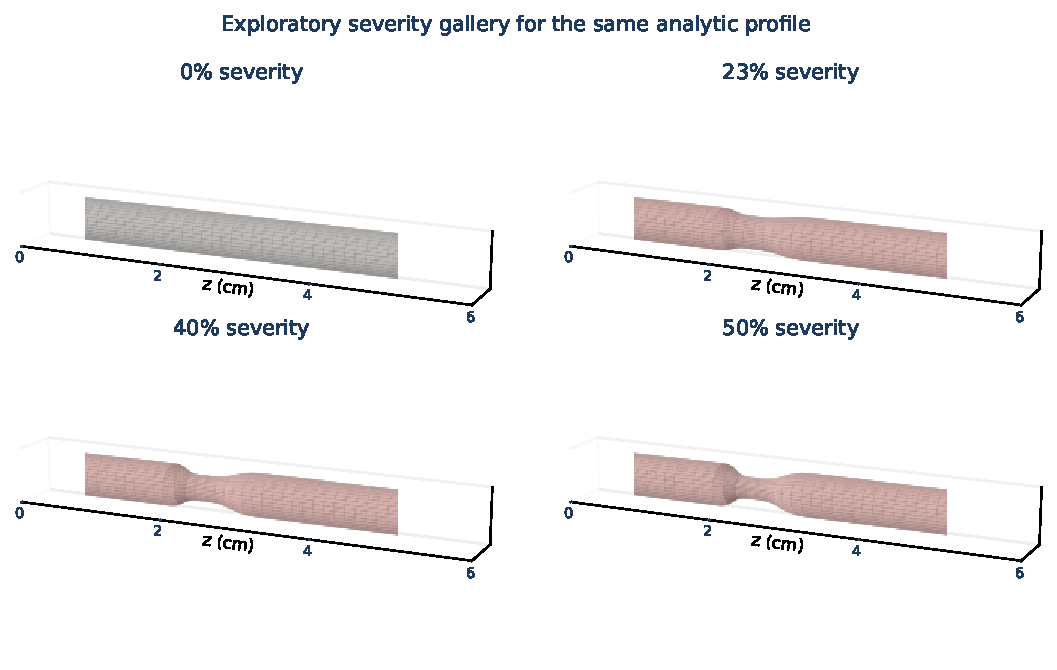
\includegraphics[width=0.98\textwidth]{figures/static/static/rendered/stenosis-severity-gallery.pdf}
    \caption{Analytic three-dimensional renderings of the
    \(C^\infty\) reference geometry in
    Definition~\ref{def:1d-stenosis-reference-geometry}, shown for
    \(s_{\max}=0\%,23\%,40\%,50\%\). Here \(s_{\max}\) is the prescribed
    anatomical radius-reduction parameter in the idealized geometry. These
    renderings illustrate the geometry family only; they are not pressure-drop,
    FFR, or patient-specific clinical calibration measurements.}
    \label{fig:stenosis-3d-reference-geometry}
\end{figure}

\begin{remark}[Stenosis-profile and variable-radius boundary]
    \label{rmk:1d-stenosis-profile-scope}
    The profile in Eq.~\ref{eq:1d-stenosis-profile} is \(C^\infty\) and
    rapidly localized rather than compactly supported. This smooth idealized
    geometry is the baseline for the reduced simulations in this report. Canic
    et al. show that standard 1D variable-geometry models may miss stenotic
    pressure and velocity trends unless additional variable-radius terms are
    included \cite[Abstract; Secs.~1--2]{CanicEtAl2024Extended1DStenosis}.
    Those corrections motivate later comparison questions, but they are not
    active in the baseline model unless a separate closure identifier and
    numerical contract are declared.
\end{remark}

\begin{definition}[Conservative flux/source notation for the reduced wall law]
    \label{def:1d-conservative-flux-source-notation}
    For a reduced wall closure \(\mathcal W\) admitting an elastic potential,
    define
    \begin{flalign*}
        \quad
        \mathbf U
        &=
        (A,Q)^\top, &&
        \mathbf F_{\mathcal W}(\mathbf U,z,t)
        =
        \begin{pmatrix}
            Q\\[2pt]
            \alpha Q^2/A+\Psi_{\mathcal W}(A,z,t)
        \end{pmatrix}, &&\\
        \quad
        \mathbf S_{\mathcal W,\mathcal R}(\mathbf U,z,t)
        &=
        \begin{pmatrix}
            0\\[2pt]
            S_{\mathrm{geom}}^{\mathcal W}(A,z,t)
            +S_f^{\mathcal R}(A,Q,z)
        \end{pmatrix}. &&
    \end{flalign*}
    The potential and sources are tied to the selected closure descriptors by
    \begin{flalign*}
        \quad
        \pd_A \Psi_{\mathcal W}(A,z,t)
        &=
        \frac{A}{\rho} \pd_A p_{\mathrm g}^{\mathcal W}(A,z,t), &&\\
        \quad
        S_{\mathrm{geom}}^{\mathcal W}(A,z,t)
        &=
        \left.\pd_z \Psi_{\mathcal W}(A,z,t)\right|_A
        -
        \frac{A}{\rho}
        \left.\pd_z p_{\mathrm g}^{\mathcal W}(A,z,t)\right|_A,
        &&\\
        \quad
        S_f^{\mathcal R}(A,Q,z)
        &=
        -C_f^{\mathcal R}(z,A,Q)\frac{Q}{A}. &&
    \end{flalign*}
    For \(\mathcal W_{\mathrm{elastic1D}}\),
    \(p_{\mathrm g}^{\mathcal W}\) is the wall law in
    Definition~\ref{def:1d-elastic-wall-law}. In component form,
    \begin{flalign*}
        \quad \pd_t A + \pd_z Q &= 0,
        \numberthis\label{eq:1d-conservative-mass} && \\
        \quad \pd_t Q
        + \pd_z \left(
            \alpha\frac{Q^2}{A}+\Psi_{\mathcal W}(A,z,t)
        \right)
        &=
        S_{\mathrm{geom}}^{\mathcal W}(A,z,t)
        +S_f^{\mathcal R}(A,Q,z),
        \numberthis\label{eq:1d-conservative-momentum} &&
    \end{flalign*}
    The wall/FSI descriptor \(\mathcal W\) determines the pressure--area law,
    elastic potential, wave speed, and geometry source; the rheology descriptor
    \(\mathcal R\) determines the viscosity or friction hook. A resolved FSI
    model is therefore not obtained by merely relabeling
    \(S_{\mathrm{geom}}\): it introduces structural state and interface laws.
    The displayed split records the balance-law objects needed by finite-volume
    schemes, while a computed realization may still use a particular
    well-balanced or source-split discretization
    \cite{LeVeque2002FiniteVolumeMethodsForHyperbolicProblems}
    \cite[Summary; Secs.~2.1--2.3; Secs.~5--6]{BoileauEtAl2015Benchmark}
    \cite{FormaggiaEtAl2007FSICoupling}.
\end{definition}

\begin{definition}[Single-vessel boundary data]
    \label{def:1d-single-vessel-boundary-data}
    For a single-vessel solve on \(z\in[0,L]\), prescribe one inlet condition
    and one outlet condition:
    \begin{flalign*}
        \quad Q(0,t) &= Q_{\mathrm{in}}(t)
        \quad \text{or} \quad
        \bar u(0,t) = \bar u_{\mathrm{in}}(t), && \\
        \quad p_{\mathrm g}(L,t) &= p_{\mathrm{out},\mathrm g}(t)
        \quad \text{or} \quad
        p_{\mathrm g}(L,t) = p_{\mathrm{WK,g}}(Q(L,\cdot),t). &&
    \end{flalign*}
    The second outlet option denotes a terminal Windkessel-style relation. The
    first controlled study uses prescribed \(Q_{\mathrm{in}}(t)\) and
    \(p_{\mathrm{out},\mathrm g}(t)\) because they give an unambiguous reduced
    single-vessel contract.
\end{definition}

\begin{assumption}[Subcritical boundary regime]
    \label{ass:1d-subcritical-boundary-regime}
    The baseline boundary treatment is used only in the subcritical regime
    \(\lambda_-<0<\lambda_+\), where one characteristic enters through the inlet
    and one characteristic enters through the outlet.
\end{assumption}

Under this regime, a finite-volume scheme constrains the incoming
information at each boundary and leaves the outgoing state determined by the
interior solve. This is the reduced-model analogue of declaring enough boundary
data for the selected equation class; it is not, by itself, a validation of a
particular boundary discretization.

\subsubsection{Model Hierarchy and Comparison Boundary}
\label{subsubsec:model-hierarchy}

Reduced hemodynamic models form a hierarchy of modeling roles rather than a
simple accuracy ranking. A higher-dimensional model becomes a comparison only
after the kinematic and continuum assumption package, geometry, wall response,
rheology, inlet and outlet data, numerical resolution, output operators, and
discrepancy metrics are matched.

\begin{figure}[!htb]
    \centering
    \captionsetup{aboveskip=2pt,belowskip=2pt}
    \figtikz{model-hierarchy}
    \caption{Model hierarchy for reading comparison claims. The present
    manuscript selects a 1D reduced forward model; 3D fixed-wall, resolved FSI,
    clinical, and independent-solver comparisons require separately matched
    evidence.}
    \label{fig:model-hierarchy-overview}
\end{figure}

\begin{table}[!htb]
    \centering
    \scriptsize
    \caption{Hemodynamic model taxonomy for the idealized stenosis report.}
    \label{tab:literature-model-taxonomy}
    \begin{tabularx}{\textwidth}{@{}
        >{\raggedright\arraybackslash}p{0.17\textwidth}
        >{\raggedright\arraybackslash}X
        >{\raggedright\arraybackslash}X
        >{\raggedright\arraybackslash}X
        @{}}
        \toprule
        \textbf{Model family}
            & \textbf{Typical role}
            & \textbf{Common states or outputs}
            & \textbf{Report boundary} \\
        \midrule
        0D lumped circulation
            & Outlet loads, Windkessel context, and network hemodynamic summaries
            & Compartment pressures, flows, resistances, compliances, inertances
            & Useful for boundary conditions, not for local stenosis geometry or
            resolved wall traction \\
        Classical 1D compliant-vessel models
            & Distributed area-flow description after cross-sectional averaging
            & \(A(z,t)\), \(Q(z,t)\), \(p_{\mathrm g}(z,t)\), wave speed, pressure drop
            & Main reduced model tier under declared continuum, wall, friction,
            inlet, and outlet assumptions \\
        Stenosis-aware 1D and pressure-loss ROMs
            & Idealized stenosis trends, variable-radius corrections, or algebraic
            loss estimates
            & Stenosis profile, severity, flow rate, \(\Delta p\), pressure ratio,
            reduced shear proxy
            & Reduced-order trend context only unless matched against resolved or
            clinical evidence \\
        2D/3D fixed-wall and resolved-FSI models
            & Higher-fidelity local flow and wall-motion comparison
            & Velocity, pressure, wall traction, WSS, wall displacement, mesh and
            time diagnostics
            & Reference-tier context unless the same continuum setting,
            geometry, rheology, wall, boundary data, and outputs are compared
            directly \\
        Numerical reference problems for 1D solvers
            & Scheme comparison, reproducibility expectations, and implementation
            context
            & Grid, timestep, flux and source choices, boundary states, field and
            scalar discrepancies
            & Evidence standard; does not grant solver parity to the present code
            without a matched comparison \\
        \bottomrule
    \end{tabularx}
\end{table}

The table should be read together with
Definition~\ref{def:wall-fsi-closure-catalog}. Spatial dimension and wall
coupling are separate choices: a 3D computation can be fixed-wall or resolved
FSI, and a 1D computation can be rigid-tube, elastic-wall, or coupled to
upstream/downstream models. Consequently, an FSI comparison claim requires the
wall descriptor \(\mathcal W\), rheology descriptor \(\mathcal R\), boundary
data, interface conditions, and output operators to be matched; it does not
follow from the flux/source notation or from model dimension alone.

Across these categories, the recurring descriptors are the kinematic/continuum
setting, stenosis geometry, wall stiffness or compliance, density, viscosity or
effective-viscosity law, inlet waveform, outlet pressure or load,
pressure-reference convention, and tap locations. The recurring outputs are
pressure drop, reduced pressure ratio, area, flow, radius, and either a reduced
wall-friction/shear proxy or a resolved traction-based WSS quantity
\cite{ShiEtAl2011BloodFlowModelReview,FormaggiaEtAl2003OneDimensionalBloodFlow,KopplHelmig2023DimensionReducedModeling}
\cite{CanicEtAl2024Extended1DStenosis,FormaggiaEtAl2007FSICoupling}.
The report therefore treats the selected 1D area-flow model as the controlled
forward map for the first numerical study, while reserving 3D/FSI agreement,
clinical calibration, and independent-solver parity for later evidence.

\subsubsection{3D Fixed-Wall and Resolved-FSI Models}
\label{subsubsec:3d-models}

A fixed-wall 3D hemodynamic model solves for the velocity field
$\vu(t,\vx)$, pressure field $p(t,\vx)$, and stress-derived outputs on a
three-dimensional lumen with fixed or prescribed wall geometry
\cite{QuarteroniFormaggia2004CardiovascularModeling}. It can supply resolved
velocity, pressure, and wall traction. A WSS output additionally requires the
stress tensor, wall normal, wall location, tangent convention, and output
operator to be declared
\cite{JohnEtAl2017WallShearStressVectorForm}. These quantities are fields on
the resolved lumen and describe the vessel wall's interaction with the fluid
domain, not the 1D state variables $A$, $Q$, and $p_{\mathrm g}$.

Resolved FSI changes the wall descriptor. A fixed-wall model belongs to the
$\mathcal W_{\mathrm{rigid}}$ or prescribed-wall reading in
Definition~\ref{def:wall-fsi-closure-catalog}; a resolved-FSI model uses
$\mathcal W_{\mathrm{resolvedFSI}}$ and adds wall displacement, wall velocity,
structural stress, and fluid--structure interface conditions. The elastic 1D
wall law $\mathcal W_{\mathrm{elastic1D}}$ is a reduced wall closure, not a
structural FSI solve
\cite{FormaggiaEtAl2007FSICoupling}.

The 3D/FSI tier can represent eccentricity, curvature, branches, secondary
flow, separation, and recirculation more directly than a 1D area--flow model.
That role does not make it assumption-free. A valid comparison requires matched
geometry, rheology descriptor $\mathcal R$, wall closure $\mathcal W$, boundary
data, mesh and time resolution, output operators, and discrepancy metrics. A
velocity-slab diagnostic, a traction-based WSS comparison, and a pressure-ratio
comparison are different observation problems.

The 3D/FSI tier supplies the reference vocabulary for resolved velocity,
pressure, traction, and wall motion, but it does not automatically validate a
reduced model without matched comparison data. It is not the selected broad
parametric generator in this report because the setup and computational burden
are high, not because resolved 3D or FSI models are unimportant.

\subsection{Model Hierarchy and Comparison Boundary}
\label{subsec:model-hierarchy-comparison-boundary}

Reduced hemodynamic models form a hierarchy of modeling roles rather than a
scalar accuracy ranking. The governing equations above start from a
three-dimensional continuum problem and then introduce reduced descriptions, so
this subsection reads the hierarchy in descending spatial dimension. Dimension,
wall treatment, rheology, boundary data, coupling laws, output operators, and
numerical realization remain separate modeling choices. This report selects the
1D area--flow model as the reduced forward map; 3D, multiscale, 2D, and 0D
models supply comparison, coupling, diagnostic, and boundary-condition
vocabulary.

\begin{figure}[!htb]
    \centering
    \captionsetup{aboveskip=2pt,belowskip=2pt}
    \figtikz{model-hierarchy}
    \caption{Model hierarchy for reading comparison claims, ordered from the
    three-dimensional continuum tier toward reduced and lumped closures. The
    horizontal direction is a dimensional-reduction and closure-abstraction
    axis, not a validation ranking. This report selects a 1D reduced forward
    model; 3D fixed-wall, resolved FSI, clinical, and independent-solver
    comparisons require separately matched assumptions, inputs, output
    operators, and discrepancy metrics before they can support evidence claims.}
    \label{fig:model-hierarchy-overview}
\end{figure}

\begin{definition}[Wall and coupling closure axes]
    \label{def:wall-fsi-closure-catalog}
    The wall descriptor $\mathcal W$ records how the wall or wall-reduced
    mechanics are closed. The coupling descriptor $\mathcal C$ records whether
    the single vessel is isolated or coupled to another model tier. Both are
    independent of the rheology descriptor $\mathcal R$: $\mathcal R$ changes
    the stress or effective-viscosity law, $\mathcal W$ changes the wall
    mechanics, and $\mathcal C$ changes the interface or network contract.
    \begin{center}
    \footnotesize
    \begin{tabularx}{\textwidth}{@{}
        >{\raggedright\arraybackslash}p{0.17\textwidth}
        >{\raggedright\arraybackslash}p{0.18\textwidth}
        >{\raggedright\arraybackslash}X
        >{\raggedright\arraybackslash}X
        @{}}
        \toprule
        \textbf{Axis}
            & \textbf{Descriptor}
            & \textbf{Information retained}
            & \textbf{Reading in this report} \\
        \midrule
        Wall
            & $\mathcal W_{\mathrm{rigid}}$
            & Fixed or prescribed wall geometry; no structural state is solved
            & A fixed-wall continuum or rigid-tube reduced baseline. \\
        Wall
            & $\mathcal W_{\mathrm{elastic1D}}$
            & Dynamic area $A(z,t)$, gauge pressure $p_{\mathrm g}(A,z,t)$,
            reference area $A_0(z)$, wall stiffness $\beta(z)$, and external
            pressure
            & A pressure--area wall-law family. The selected 1D model below
            uses its Canic--Koiter member; no separate structural PDE is
            solved. \\
        Wall
            & $\mathcal W_{\mathrm{resolvedFSI}}$
            & Fluid velocity and pressure plus wall displacement, wall velocity,
            structural stress, and interface conditions
            & A full moving-wall FSI PDE system, used here only as comparison
            vocabulary. \\
        Coupling
            & $\mathcal C_{\mathrm{isolated}}$
            & Inlet and outlet data close one vessel
            & The baseline numerical study. \\
        Coupling
            & $\mathcal C_{\mathrm{network}}$ or $\mathcal C_{\mathrm{3D/1D}}$
            & Interface pressure, flow, traction, impedance, or characteristic
            data connecting 0D, 1D, and 3D tiers
            & A separate boundary/interface contract, not a wall law. \\
        \bottomrule
    \end{tabularx}
    \end{center}
    This separation follows the standard distinction between reduced compliant
    vessel models, geometrical multiscale coupling, and resolved FSI models
    \cite[Sec.~2, pp.~253--257]{FormaggiaEtAl2003OneDimensionalBloodFlow}
    \cite{QuarteroniVeneziani2003GeometricalMultiscale}
    \cite{FormaggiaEtAl2007FSICoupling}.
\end{definition}

\subsubsection{3D Fixed-Wall and Resolved-FSI Models}
\label{subsubsec:3d-models}

A fixed-wall 3D hemodynamic model solves for the velocity field
$\vu(t,\vx)$, pressure field $p(t,\vx)$, and stress-derived outputs on a
three-dimensional lumen with fixed or prescribed wall geometry
\cite{QuarteroniFormaggia2004CardiovascularModeling}. It can supply resolved
velocity, pressure, and wall traction. A WSS output additionally requires the
stress tensor, wall normal, wall location, tangent convention, and output
operator to be declared
\cite{JohnEtAl2017WallShearStressVectorForm}. These quantities are fields on
the resolved lumen and describe the vessel wall's interaction with the fluid
domain, not the 1D state variables $A$, $Q$, and $p_{\mathrm g}$.

Resolved FSI changes the wall descriptor. A fixed-wall model belongs to the
$\mathcal W_{\mathrm{rigid}}$ or prescribed-wall reading in
Definition~\ref{def:wall-fsi-closure-catalog}; a resolved-FSI model uses
$\mathcal W_{\mathrm{resolvedFSI}}$ and adds wall displacement, wall velocity,
structural stress, and fluid--structure interface conditions. The elastic 1D
wall law $\mathcal W_{\mathrm{elastic1D}}$ is a reduced wall closure, not a
structural FSI solve
\cite{FormaggiaEtAl2007FSICoupling}.

The 3D/FSI tier can represent eccentricity, curvature, branches, secondary
flow, separation, and recirculation more directly than a 1D area--flow model.
That role does not make it assumption-free. A valid comparison requires matched
geometry, rheology descriptor $\mathcal R$, wall closure $\mathcal W$, boundary
data, mesh and time resolution, output operators, and discrepancy metrics. A
velocity-slab diagnostic, a traction-based WSS comparison, and a pressure-ratio
comparison are different observation problems.

The 3D/FSI tier supplies the reference vocabulary for resolved velocity,
pressure, traction, and wall motion, but it does not automatically validate a
reduced model without matched comparison data. It is not the selected broad
parametric generator in this report because the setup and computational burden
are high, not because resolved 3D or FSI models are unimportant.

\subsubsection{Multiscale 3D--1D--0D Coupling}
\label{subsubsec:multiscale-models}

A multiscale model is a coupled forward problem that combines tiers of the
hierarchy. A common arrangement resolves a local 3D stenosis region, connects it
to a surrounding 1D distributed vessel network, and closes terminal beds with
0D Windkessel or related outlet models. The purpose is to keep local resolved
physics where it matters while representing wave propagation and distal
impedance without making the entire circulation a 3D domain
\cite{QuarteroniVeneziani2003GeometricalMultiscale}.

The interface laws are part of the model. A 3D--1D interface may impose
conservation of flow together with pressure, mean-pressure, normal-traction, or
characteristic compatibility. A 1D--0D interface passes terminal flow into an
ODE load and returns a pressure or impedance relation to the 1D boundary.
Resolved-FSI coupling additionally requires compatible wall kinematics,
structural stresses, and interface work. These choices affect stability and
interpretation, and they must be recorded with the numerical coupling convention
\cite{FormaggiaEtAl2007FSICoupling}.

A multiscale model is not a new fidelity tier; it is a coupled forward problem
whose interface laws are part of the model definition. Coupling more components
does not automatically make a comparison more correct. The boundary data,
interface variables, time coupling, output maps, and discrepancy metrics decide
what claim the computation can support. In this report, multiscale coupling
provides comparison and boundary-condition vocabulary; it is not the active
baseline single-vessel solve unless explicitly declared.

\subsubsection{2D Intermediate Resolved-Flow Models}
\label{subsubsec:2d-models}

A 2D model is treated here as a conceptual intermediate resolved-flow tier,
usually posed as an axisymmetric or planar flow problem. It retains a spatially
resolved velocity and pressure field on an idealized reduced domain rather than
only the section-averaged state $(A,Q,p_{\mathrm g})$. Within those
idealizations, it can be used to inspect radial velocity structure, throat
acceleration, simplified recirculation, and wall-shear trends that a 1D
area--flow model cannot resolve.

The same idealization also fixes the boundary of the evidence. Axisymmetric and
planar models suppress eccentric plaques, curvature, torsion, branch geometry,
non-axisymmetric secondary flow, and fully patient-specific WSS\@. Their wall
outputs depend on the declared stress tensor, wall location, normal, tangent,
and output operator, just as in the shear convention of
Convention~\ref{conv:appendix-shear-diagnostic}. A 2D result is therefore not
interchangeable with matched 3D or resolved-FSI evidence. The broad continuum
and dimension-reduction background for this reading is supplied by
\cite{GaldiEtAl2008HemodynamicalFlows,KopplHelmig2023DimensionReducedModeling}.

The 2D tier is a diagnostic bridge: useful for controlled mechanism checks, but
too idealized to serve as clinical or resolved-3D evidence. In this report it
can help interpret whether a reduced trend is plausibly tied to throat
acceleration or simplified recirculation, but it is not the selected forward
generator and does not validate the 1D map by itself.

\subsubsection{1D Distributed Area--Flow Models}
\label{subsubsec:1d-models}

The selected 1D reduction is defined in
Section~\ref{subsubsec:cross-sectional-reduction-selected-1d-model}. There the
retained fields $A(z,t)$, $Q(z,t)$, $\bar u(z,t)=Q/A$, and
$p_{\mathrm g}(z,t)$, the wall and coupling closure catalog, the elastic-wall
area--flow balance law, the stenosis reference geometry, the conservative
flux/source notation, and the single-vessel boundary data are recorded in
Definitions~\ref{def:section-averaged-1d-fields}--\ref{def:1d-single-vessel-boundary-data}
\cite{FormaggiaEtAl2003OneDimensionalBloodFlow,KopplHelmig2023DimensionReducedModeling}.
This subsection uses that machinery only to identify the hierarchy role of the
1D tier.

In the hierarchy, the key point is that the 1D state is distributed but reduced.
It retains axial area, flow, mean velocity, and gauge pressure; it does not
retain the full three-dimensional velocity field, pressure field, secondary
flow, separation, recirculation, or wall traction. Reduced shear quantities
therefore inherit the declared velocity-profile, wall-friction, and rheology
closures. They are not traction-based WSS unless a separate observation map
declares how a reduced output is compared with a resolved wall-stress quantity.

The closure contract remains part of the model definition. A 1D case must
declare the momentum-flux/profile convention, friction law, rheology descriptor
$\mathcal R$, wall descriptor $\mathcal W$, boundary data, numerical
realization, and output operators. Stenosis enters through the reference
geometry $R_0(z)$, $A_0(z)$, and $s(z)$, but resolved throat flow does not
appear automatically; variable-radius corrections such as the Canic-style terms
are additional closure choices
\cite{CanicEtAl2024Extended1DStenosis}.
The current implementation records this axis explicitly through the
\texttt{canic-extended-1d} and \texttt{classical-1d-no-slip} forward-model
descriptors, the latter corresponding to the wall no-slip baseline in
Definition~\ref{def:classical-no-slip-1d-baseline}.

The 1D model is the selected reduced forward map because it retains distributed
pressure--flow structure at low computational cost, while its outputs remain
reduced quantities with declared observation maps. In this report it is the
selected single-vessel generator for the numerical study, not a
clinical-validation claim, an independent-solver parity claim, or a
resolved-3D-accuracy claim.

\subsubsection{0D Outlet and Network Models}
\label{subsubsec:0d-models}

A 0D model is a lumped ODE or circuit model for pressures, flows, volumes, and
loads. It retains compartment pressures, branch flows, resistances,
compliances, and, when the circuit includes inertial effects, inertances. The
model preserves a time-dependent pressure--flow relation for parts of the
circulation that are not spatially resolved. Windkessel and RCR models are the
canonical terminal examples: they supply an outlet impedance or downstream load
for a local 1D or 3D vessel solve
\cite{ShiEtAl2011BloodFlowModelReview,KopplHelmig2023DimensionReducedModeling}.

A 0D model closes the circulation seen by the local vessel model; it does not
resolve the local stenosis. The spatial coordinate has been integrated out, so
the model has no local stenosis geometry, no axial pressure-drop field, no
throat acceleration profile, and no recirculation region. It also has no
resolved wall-shear stress or wall traction, because it does not carry a lumen
surface, a stress tensor on that surface, or a wall-normal output operator.

The 0D tier is therefore useful boundary and network context for this report. It
can prescribe an outlet load, organize distal-bed assumptions, or provide a
lumped circulation closure. It is not the selected local stenosis-resolution
tier and cannot replace the distributed area--flow state used in the numerical
study in this report.


A comparison claim requires matched assumptions and declared output operators:
the continuum setting, geometry, rheology descriptor $\mathcal R$, wall
descriptor $\mathcal W$, coupling descriptor $\mathcal C$, boundary data,
numerical settings, observation maps, and discrepancy metrics must all be part
of the comparison record. This report treats the selected 1D area--flow model
as the forward map for the numerical study. Resolved-3D/FSI agreement, clinical
calibration, and independent-solver parity are later evidence standards, not
assumptions built into the model hierarchy.


\subsection{One-Dimensional Modelling of Nonuniform and Stenotic Vessels}
\label{subsec:literature-1d-stenotic-vessels}

The stenotic-vessel setting is the point at which the reduced-model assumptions
become especially visible. Cross-sectional averaging replaces the resolved
velocity field by $A(z,t)$, $Q(z,t)$, a mean velocity, and a pressure variable.
That reduction requires a velocity-profile or momentum-flux closure, a wall law
or wall descriptor, a friction/rheology convention, and a rule for how variable
geometry enters the momentum balance. These choices are not interchangeable:
changing a wall law, changing a profile factor, and adding a variable-radius
source correction change different parts of the model.

\subsubsection{Cross-Sectional Averaging and Closure Assumptions}

One-dimensional area--flow models retain distributed axial information while
discarding secondary flow, skewed profiles, separation, and recirculation. The
lost transverse information re-enters only through closures such as the
momentum-flux correction factor, profile reconstruction rule, and wall-friction
term. This is why a comparison with resolved 3D data must state the observation
operator before interpreting any difference between the two outputs.

\subsubsection{Wall and Constitutive Laws}

The wall descriptor determines whether the model uses a fixed geometry, an
algebraic pressure--area relation, a coupled network/interface condition, or a
resolved structural model. The rheology descriptor separately controls the
viscosity or effective-viscosity law. In the selected study, these axes remain
separate: the working 1D model uses an elastic pressure--area wall law and a
declared rheology/profile closure, while resolved FSI remains a different
model tier rather than a relabelled source term.

\subsubsection{Variable Geometry and Stenosis Corrections}

Stenosis enters a one-dimensional model through the reference radius or
reference area, but a narrowed geometry by itself does not determine the
correct reduced momentum equation. Variable-radius terms, wall-source balance,
and profile corrections must be part of the stated model. This report therefore
distinguishes the classical parabolic-profile baseline from the
\texttt{canic-extended-1d} member that includes the Canic-style
variable-radius corrections.

\subsubsection{Known Limitations of One-Dimensional Stenosis Models}

A 1D model cannot resolve eccentricity, three-dimensional separation,
recirculation, secondary flow, or traction-based wall shear stress. It can still
be useful when the output of interest is a declared area--flow or
section-averaged velocity quantity. The limitation is evidential rather than
cosmetic: agreement in a section mean would not prove resolved velocity
agreement, and disagreement in a section mean would not by itself identify a
single physical mechanism.

\subsection{Numerical Verification and Cross-Dimensional Comparison}
\label{subsec:verification-comparison-background}

Verification, cross-model comparison, and validation answer different
questions. Verification asks whether the implemented equations and numerical
operators behave consistently under declared checks. Cross-model comparison
asks how two computational outputs differ under a stated observation operator.
Validation asks whether a model reproduces independent physical, experimental,
or clinical measurements. This report uses the first two categories only.

\subsubsection{Verification of One-Dimensional Solvers}

For a reduced 1D solver, relevant verification evidence includes descriptor
checks, boundary diagnostics, self-convergence, cross-integrator discrepancy,
mass/positivity/CFL diagnostics, and reproducible output schemas. Such evidence
supports claims about the implementation and numerical record. It does not by
itself establish physiological pressure accuracy or clinical validity.

\subsubsection{Comparison with Resolved Three-Dimensional Data}

A resolved 3D comparison can be informative only after the observable has been
defined. The report therefore treats plane--tetrahedron quadrature of axial
velocity as an output operator from the resolved field to section-averaged
quantities comparable with the 1D solution. The comparison remains bounded by
the available metadata: unmatched wall model, boundary histories, material
parameters, and transient histories limit attribution.

\subsubsection{Distinction Between Comparison, Verification, and Validation}

The terms are kept separate throughout the report. A green software check is
not a validation experiment. A velocity discrepancy under a declared quadrature
operator is not a pressure-drop error. A reduced pressure-ratio convention is
not an FFR or CT-FFR result unless a separate clinical measurement comparison is
specified.

\subsection{Literature Synthesis and Research Gap}
\label{subsec:literature-synthesis-gap}

The literature motivates a focused methodological gap. Stenotic flow is
geometrically local and can produce velocity structures that full-order models
represent more directly than reduced models. One-dimensional models are much
cheaper and retain distributed pressure--flow behavior, but their stenosis
predictions depend on cross-sectional averaging, wall and rheology closures,
variable-geometry terms, boundary data, and output maps. Existing verification
and comparison practice also shows that numerical consistency, cross-model
agreement, and physical validation are separate evidential claims.

The gap addressed by this report is therefore not clinical validation of a
stenosis model. It is an auditable implementation and report specification for
a selected extended 1D stenosis model, paired with an explicitly defined
operator for comparing one-dimensional and resolved three-dimensional velocity
outputs.
